\documentclass[11pt]{article}

\usepackage[margin=1in]{geometry}
\usepackage{graphicx}
\usepackage{booktabs}
\usepackage{longtable}
\usepackage{array}
\usepackage{float}
\usepackage{caption}
\usepackage{hyperref}

\graphicspath{{outputs/figures/full_png/}{../outputs/figures/full_png/}}

\hypersetup{
  colorlinks=true,
  linkcolor=blue,
  citecolor=blue,
  urlcolor=blue
}

\captionsetup{font=small, labelfont=bf}
\setlength{\parindent}{0pt}
\setlength{\parskip}{0.7em}
\emergencystretch=3em

\newcommand{\commentary}[1]{%
  \par\smallskip\noindent{\footnotesize\textit{Comment.} #1}\par\normalsize
}

\title{Python Replication Report: Zhang (2005), \textit{The Value Premium}}
\author{Matheus Porto Pimentel}
\date{June 29, 2026}

\begin{document}
\maketitle

\begin{abstract}
This report documents the current stage of a model-only replication of Zhang (2005), \textit{The Value Premium}. The central modification relative to the original replication package is computational: the routines that were previously implemented in MATLAB and Fortran were translated into a Python package with scripts for calibration, value function iteration, approximate aggregation, stationary simulation, portfolio construction, figures, and tables. The empirical-data part of the paper is not replicated here.

The report summarizes the paper, identifies three central contributions, presents the figures and tables produced by the Python full replication run, and diagnoses the main deviations from the original paper. The Python results should be read as a transparent and extensible replication layer rather than a bit-for-bit reproduction of the original MATLAB/Fortran package.
\end{abstract}

\section{Scope of the Python Translation}

The original computational code for Zhang (2005) is distributed as a mixture of MATLAB scripts and Fortran/MEX routines. In this project, those routines were translated into Python. The new code base contains modules for the benchmark calibration, Rouwenhorst discretization, the risk-free rate, value function iteration, Krusell-Smith style approximate aggregation, stationary and panel simulation, Fama-French style portfolio construction, figure generation, and model-only tables.

The full replication run documented here uses 5,000 firms, 11,000 monthly periods for the equilibrium simulation, 10,000 monthly periods for the stationary distribution simulation, 20 panel simulations of 421 monthly periods each, and a capital-choice grid with 5,000 points. The generated outputs used in this report are stored in \texttt{outputs/full\_replication}, \texttt{outputs/figures/full\_png}, and \texttt{outputs/tables/full\_model}.

The current replication is intentionally model-only. It does not attempt to rebuild the empirical CRSP/Compustat tables in the paper. The relevant comparison is therefore between the simulated model moments produced by the Python code and the model-side results reported by Zhang.

\section{Summary of the Paper}

Zhang (2005) studies why high book-to-market firms, usually called value firms, earn higher average returns than low book-to-market firms, usually called growth firms. The paper proposes a rational investment-based explanation rather than a behavioral mispricing explanation. Firms choose investment and capital dynamically in the presence of aggregate productivity risk, idiosyncratic productivity risk, and adjustment costs.

The key economic mechanism is the interaction between costly reversibility and countercyclical risk prices. Reducing capital is more expensive than expanding capital, so firms with substantial assets in place become relatively inflexible in bad aggregate states. Value firms tend to have low productivity and poor investment opportunities, so their assets in place are especially risky when the price of risk is high.

The paper shows that this mechanism can generate a positive value premium and reproduce several qualitative facts about value and growth firms. In the model, value firms invest less, have weaker profitability, carry higher book-to-market ratios, and command higher expected returns because their cash flows are more exposed to bad times.

\section{Three Central Contributions}

\textbf{Contribution 1: An investment-based explanation for the value premium.}
The paper connects expected stock returns to firms' real investment decisions. High book-to-market firms earn higher expected returns because their cash flows are tied to less flexible assets in place, especially when aggregate conditions deteriorate.

\textbf{Contribution 2: Asymmetric adjustment costs as the key operating friction.}
The model emphasizes costly reversibility: cutting capital is much more expensive than expanding it. This asymmetry generates a wedge between value and growth firms' investment policies and helps make value firms riskier in recessions.

\textbf{Contribution 3: Countercyclical risk prices amplify the mechanism.}
The stochastic discount factor makes the price of risk higher in bad aggregate states. Since value firms are relatively exposed in those states, their expected returns rise relative to growth firms.

\section{Computational Pipeline}

The translated Python pipeline follows the original MATLAB/Fortran logic:

\begin{enumerate}
  \item Calibrate monthly parameters and grids from the benchmark model.
  \item Solve the firm's dynamic problem by value function iteration.
  \item Estimate an approximate law of motion for the aggregate price using simulated equilibrium paths.
  \item Simulate the stationary distribution of firms.
  \item Simulate repeated artificial panels.
  \item Sort firms into size and book-to-market portfolios.
  \item Produce model-only figures and tables.
\end{enumerate}

The equilibrium law of motion estimated in the Python full run is
\[
  p_{t+1}
  = 0.04965
  + 0.98181 p_t
  - 0.12072 (x_t-\bar{x})
  + 0.00332 \sigma_t ,
\]
with an approximate aggregation regression \(R^2\) of 0.99957. The final value function iteration used 105 iterations, with final value error 0.000825 and final policy error 0.0.

\section{Replicated Figures}

\begin{figure}[H]
  \centering
  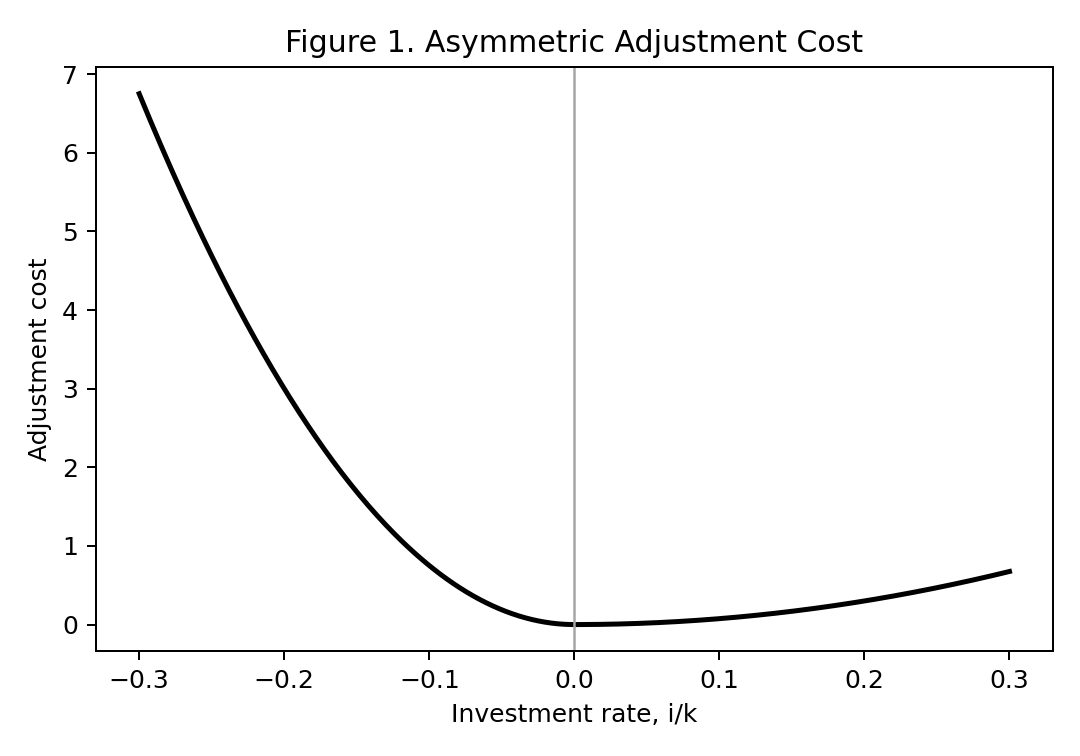
\includegraphics[width=0.86\textwidth]{figure1_adjustment_cost.png}
  \caption{Adjustment cost function}
  \label{fig:adjustment-cost}
\end{figure}
\commentary{This figure is directly tied to the second contribution. It documents the asymmetric adjustment-cost technology: positive investment is costly, but disinvestment is much more costly. The Python version reproduces the economic shape of Zhang's Figure 1 and is based on the benchmark adjustment-cost parameters used in the translated calibration.}

\begin{figure}[H]
  \centering
  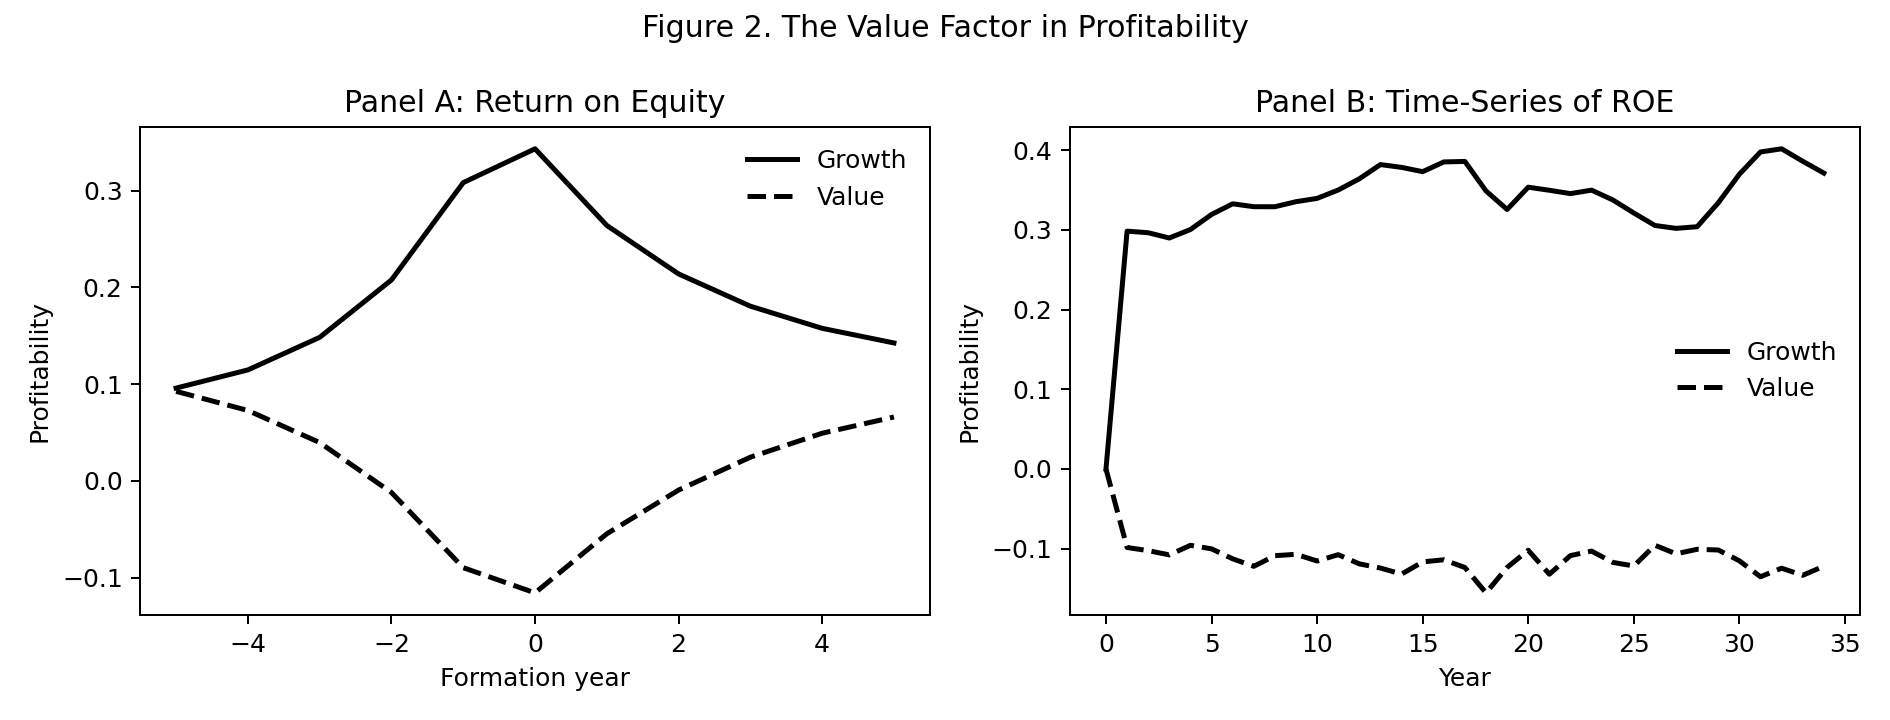
\includegraphics[width=0.86\textwidth]{figure2_ff95_profitability.png}
  \caption{Profitability patterns around portfolio formation}
  \label{fig:ff95-profitability}
\end{figure}
\commentary{This figure connects the model to the empirical-style profitability evidence emphasized in the paper. The Python implementation reconstructs the Fama-French style profitability comparison from simulated model panels. It should be interpreted as model-side evidence, not as a replication of the empirical CRSP/Compustat exercise.}

\begin{figure}[H]
  \centering
  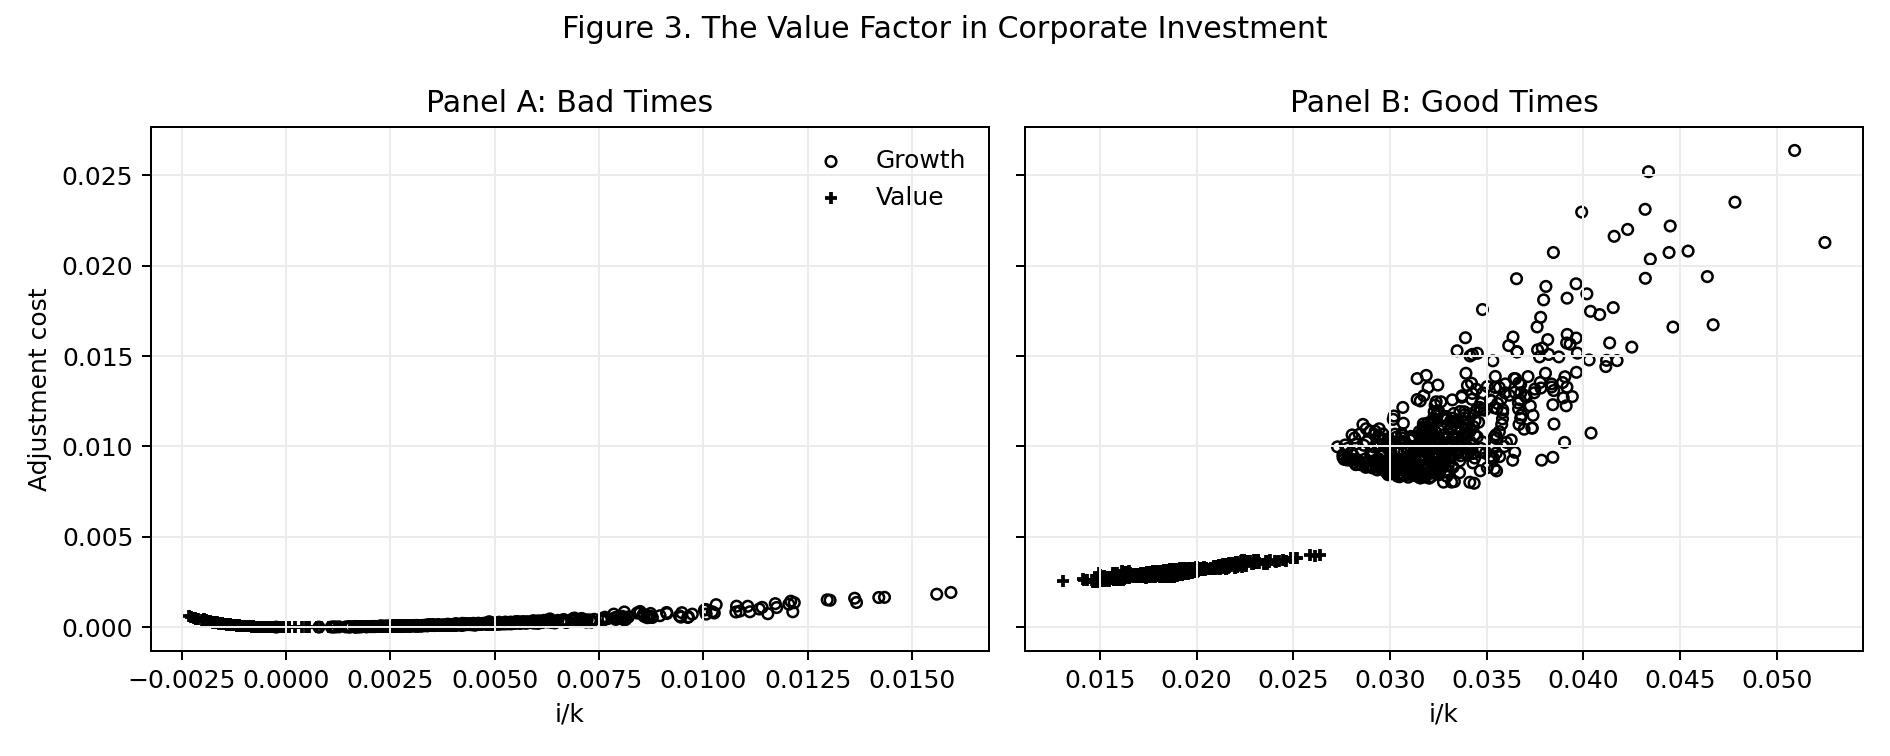
\includegraphics[width=0.86\textwidth]{figure3_investment_scatter.png}
  \caption{Investment and adjustment costs in bad and good states}
  \label{fig:investment-scatter}
\end{figure}
\commentary{This figure illustrates the investment channel behind the value premium. In the Python simulation, investment and adjustment costs vary across aggregate states and across value/growth firms. The qualitative mechanism is preserved: investment flexibility differs across firms and matters more in bad states.}

\begin{figure}[H]
  \centering
  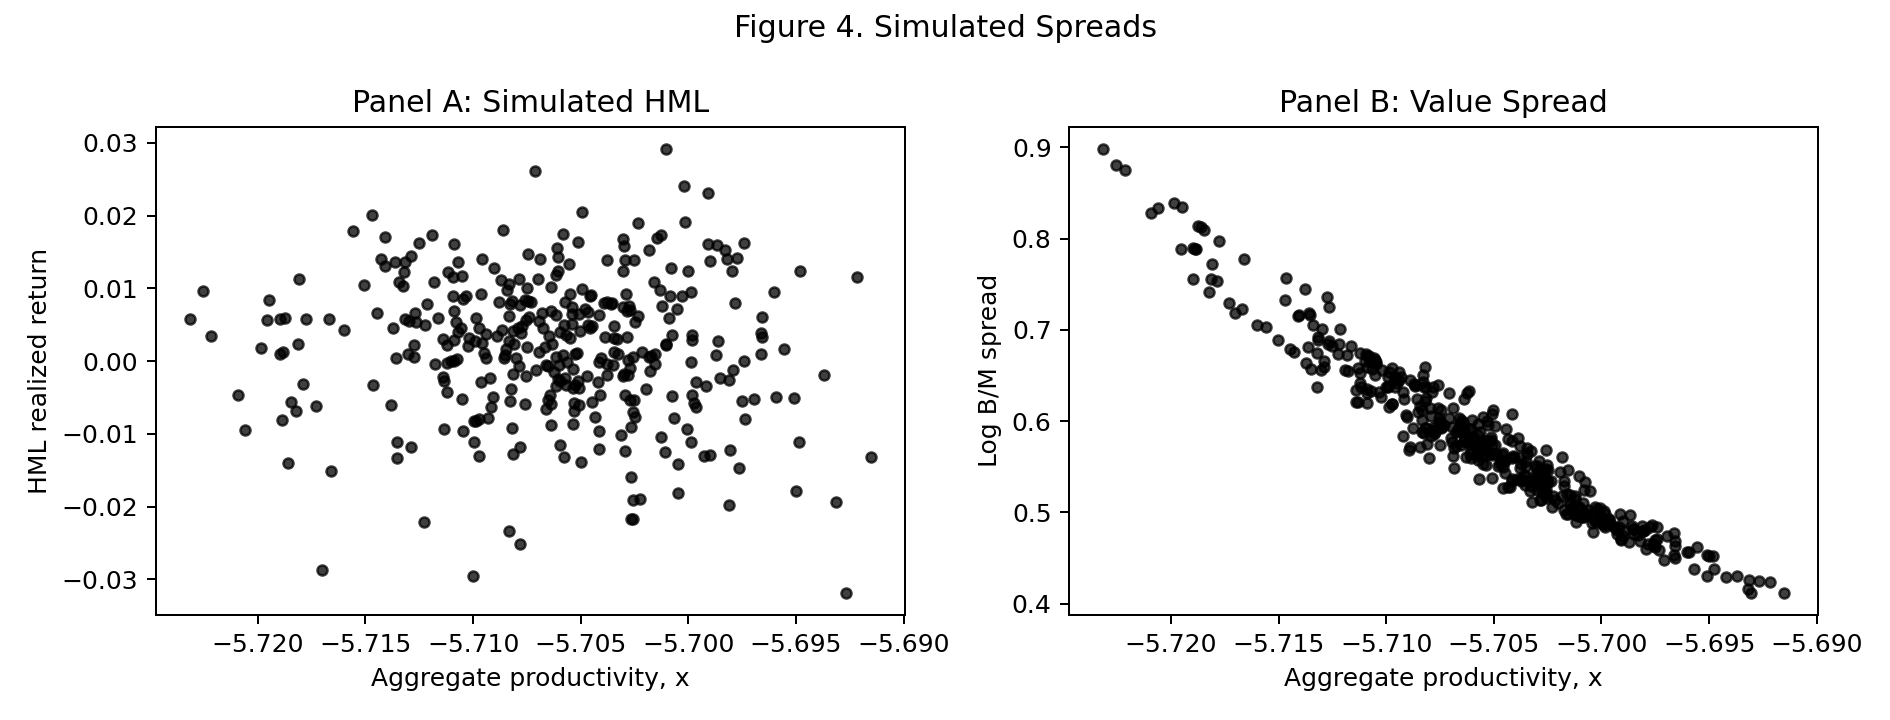
\includegraphics[width=0.86\textwidth]{figure4_simulated_spreads.png}
  \caption{Simulated value spreads and HML}
  \label{fig:simulated-spreads}
\end{figure}
\commentary{This is currently a simulated proxy for the original structural Figure 4. The value spread moves with aggregate productivity in the expected direction, but the HML panel is based on realized simulated portfolio returns rather than the exact conditional expected-return object plotted in the paper. This is one of the remaining gaps.}

\begin{figure}[H]
  \centering
  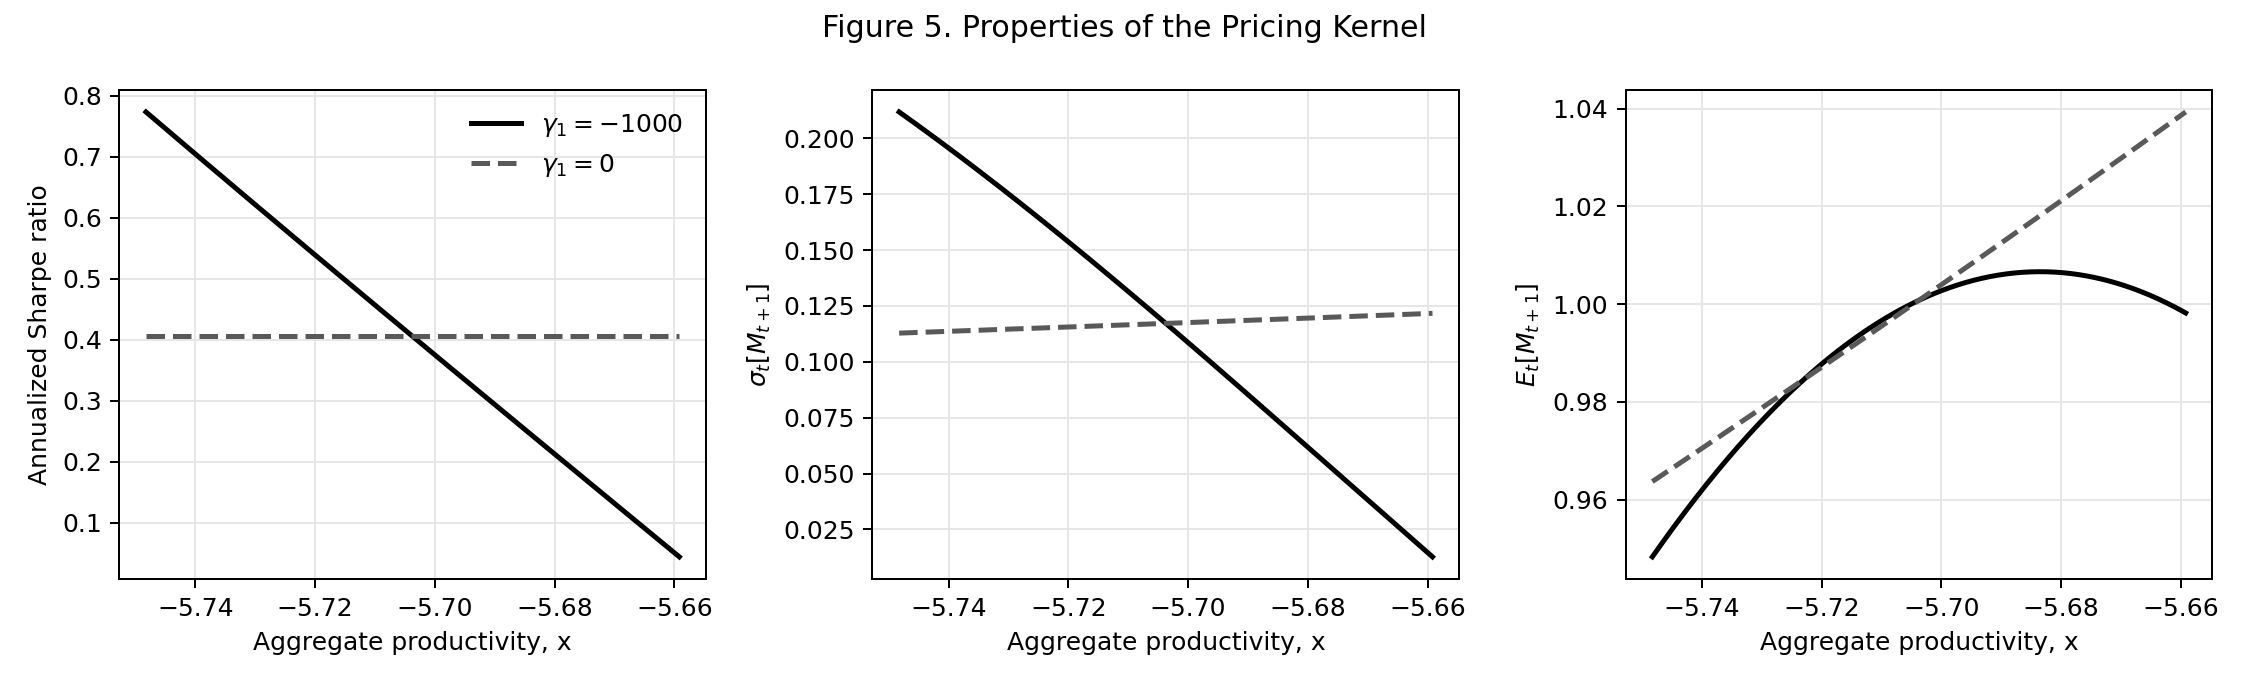
\includegraphics[width=0.86\textwidth]{figure5_pricing_kernel.png}
  \caption{Countercyclical pricing kernel}
  \label{fig:pricing-kernel}
\end{figure}
\commentary{This figure is tied to the third contribution. It shows how the benchmark stochastic discount factor makes the market price of risk larger in bad aggregate states. This countercyclical price of risk is essential for turning value firms' bad-times exposure into a return premium.}

\begin{figure}[H]
  \centering
  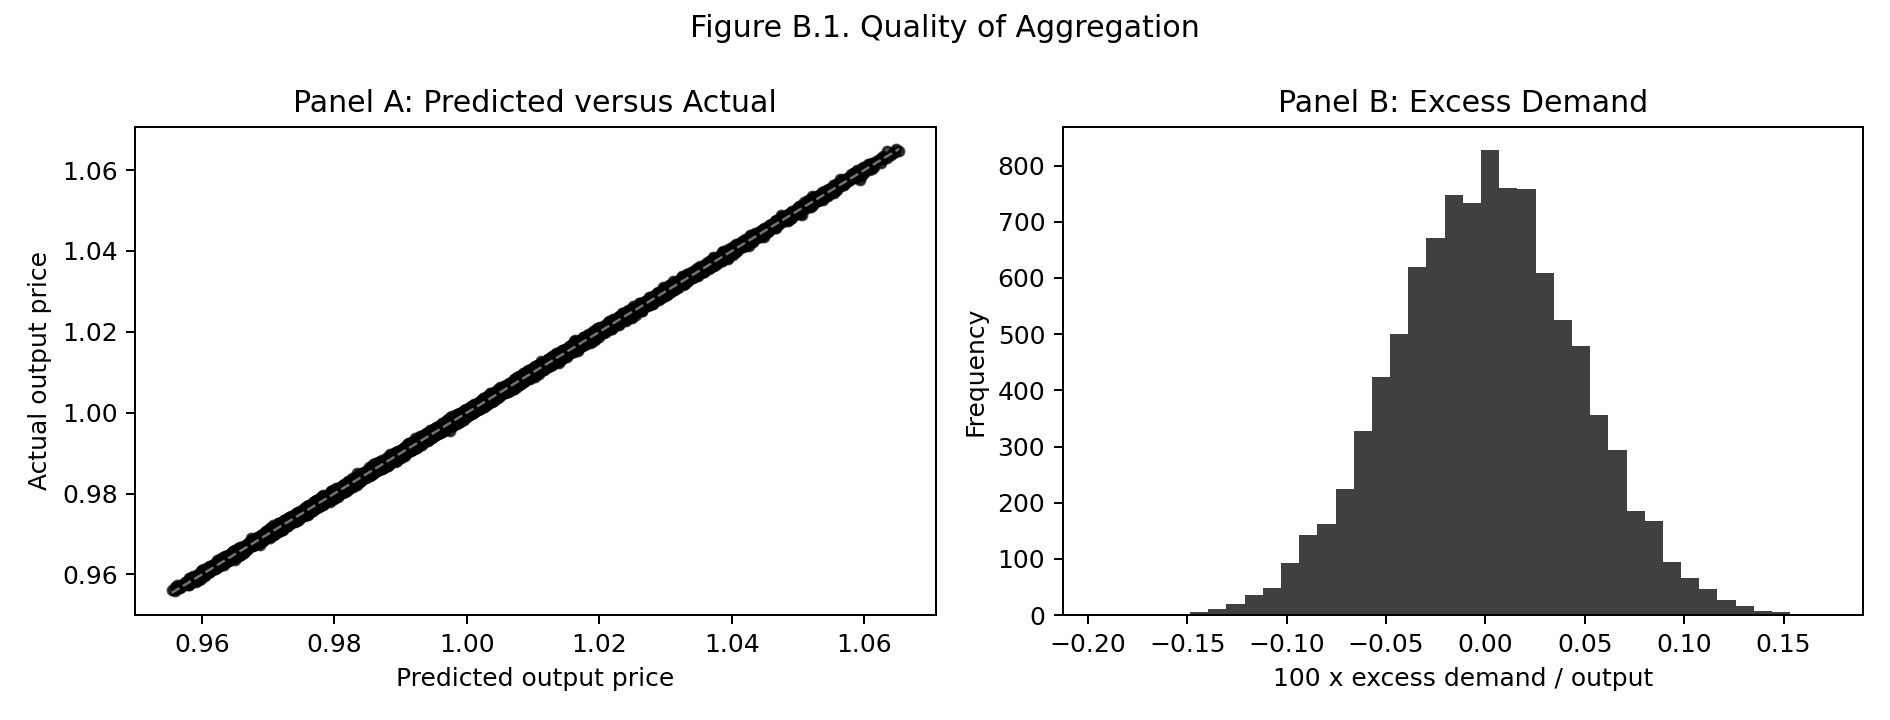
\includegraphics[width=0.86\textwidth]{figureB1_aggregation_quality.png}
  \caption{Approximate aggregation diagnostic}
  \label{fig:b1-aggregation}
\end{figure}
\commentary{This figure corresponds to the Appendix B aggregation diagnostic. In the Python full run, the aggregation residuals have mean approximately \(-2.0\times10^{-5}\), standard deviation 0.0463, and an absolute maximum below 0.20 percent of output. The fit is therefore close to the scale reported in the original approximation exercise, although the estimated coefficients are not identical to Zhang's benchmark coefficients.}

\section{Replicated Tables}

\subsection{Benchmark Parameters}

\begin{longtable}{lll}
\caption{Model parameters used in the Python full replication}
\label{tab:model-parameters}\\
\toprule
Parameter & Description & Value \\
\midrule
\endfirsthead
\toprule
Parameter & Description & Value \\
\midrule
\endhead
\bottomrule
\endfoot
\(\beta\) & Subjective discount factor & 0.994 \\
\(\gamma_0\) & Pricing kernel loading & 50 \\
\(\gamma_1\) & Countercyclical price-of-risk loading & -1000 \\
\(\eta\) & Inverse demand curvature & 0.5 \\
\(\alpha\) & Capital share & 0.3 \\
\(\delta\) & Depreciation rate & 0.01 \\
\(\theta^+\) & Adjustment cost for positive investment & 15 \\
\(\theta^-\) & Adjustment cost for negative investment & 150 \\
\(f\) & Fixed operating cost & 0.0365 \\
\(\rho_x\) & Aggregate productivity persistence & 0.983048 \\
\(\sigma_x\) & Aggregate productivity volatility & 0.00233333 \\
\(\rho_z\) & Idiosyncratic productivity persistence & 0.97 \\
\(\sigma_z\) & Idiosyncratic productivity volatility & 0.1 \\
\(N\) & Number of simulated firms & 5000 \\
\(T\) & Number of simulated monthly periods & 11000 \\
\end{longtable}
\commentary{This table documents the benchmark calibration translated from the original code. It is the foundation for all simulated figures and tables below. The parameters match the economic primitives of Zhang's model; remaining numerical differences come mostly from simulation design, implementation details, and the exact portfolio/statistic routines.}

\subsection{Key Model Moments}

\begin{table}[H]
\centering
\caption{Key model moments from the Python full replication}
\label{tab:key-moments}
\begin{tabular}{lr}
\toprule
Moment & Model \\
\midrule
Average annual Sharpe ratio & 0.405524 \\
Average annual real interest rate & 0.0134317 \\
Annual volatility of real interest rate & 0.0269625 \\
Average annual value-weighted industry return & 0.103478 \\
Annual volatility of value-weighted industry return & 0.266519 \\
Average volatility of individual stock return & 0.393690 \\
Average industry book-to-market ratio & 0.454185 \\
Volatility of industry book-to-market ratio & 0.0908488 \\
Annual average rate of investment & 0.119780 \\
Annual average rate of disinvestment & 0.00948566 \\
\bottomrule
\end{tabular}
\end{table}
\commentary{This is the corrected Python version of the model-side moments analogous to Zhang's Table II. The Sharpe ratio, risk-free rate volatility, market-return volatility, and investment rate are close in magnitude to the paper. The largest deviations are the volatility of individual stock returns, the average industry book-to-market ratio, and especially the volatility of the industry book-to-market ratio. A major reason is that the current full run uses 20 panels of 421 months, while the paper's simulation exercises use longer artificial panels and more exact summary-statistic routines.}

\subsection{Additional Model Moments}

\begin{table}[H]
\centering
\caption{Additional model moments from the Python full replication}
\label{tab:additional-moments}
\begin{tabular}{lr}
\toprule
Moment & Value \\
\midrule
Mean market excess return, annual percent & 8.55222 \\
Market return volatility, annual percent & 26.6519 \\
Mean industry book-to-market & 0.454185 \\
Volatility of industry book-to-market & 0.0908488 \\
Mean cross-sectional B/M dispersion & 0.145228 \\
Mean firm return, annual percent & 10.8205 \\
Mean firm return volatility, annual percent & 39.3690 \\
HML mean return, annual percent & 2.13074 \\
HML volatility, annual percent & 3.67143 \\
SMB mean return, annual percent & -8.69014 \\
SMB volatility, annual percent & 3.74742 \\
\bottomrule
\end{tabular}
\end{table}
\commentary{These auxiliary moments are useful diagnostics for the simulated panels. The positive HML mean confirms that the Python model generates a value premium, but the negative SMB mean is not a central target of the Zhang calibration and should not be over-interpreted without a closer replication of the original portfolio routines.}

\subsection{Book-to-Market Portfolios}

\begin{table}[H]
\centering
\caption{Book-to-market portfolios, model only}
\label{tab:bm-portfolios}
\resizebox{\textwidth}{!}{%
\begin{tabular}{lrrrrrr}
\toprule
Portfolio & Mean return & Volatility & Market beta & Beta t-stat & CAPM \(R^2\) & Mean B/M \\
\midrule
BM1 & 8.34734 & 22.7361 & 0.818184 & 425.210 & 0.997693 & 0.315633 \\
BM2 & 8.99769 & 24.6437 & 0.887994 & 470.318 & 0.998114 & 0.366693 \\
BM3 & 9.77346 & 25.6432 & 0.924370 & 484.828 & 0.998225 & 0.398456 \\
BM4 & 9.86776 & 26.6978 & 0.962793 & 504.448 & 0.998360 & 0.426634 \\
BM5 & 10.5981 & 27.7489 & 1.00120 & 532.288 & 0.998527 & 0.454448 \\
BM6 & 10.9581 & 28.7206 & 1.03683 & 526.491 & 0.998494 & 0.483992 \\
BM7 & 11.8418 & 29.9524 & 1.08148 & 518.440 & 0.998447 & 0.517852 \\
BM8 & 12.1247 & 31.5691 & 1.14023 & 459.732 & 0.998026 & 0.560291 \\
BM9 & 13.6268 & 33.5102 & 1.21060 & 409.500 & 0.997514 & 0.622716 \\
BM10 & 16.2318 & 39.1033 & 1.41170 & 264.758 & 0.994072 & 0.803702 \\
HML10 & 7.09226 & 16.7347 & 0.593513 & 86.4512 & 0.947034 & -- \\
\bottomrule
\end{tabular}}
\end{table}
\commentary{The Python simulation reproduces the main monotonic pattern behind the value premium: higher book-to-market portfolios earn higher average returns and have higher market betas. The exact magnitudes should be treated cautiously because this table still depends on simplified portfolio-summary code relative to the original \texttt{SummStats.m} and related routines.}

\subsection{Predictive Regressions}

\begin{table}[H]
\centering
\caption{Predictive regressions, model only}
\label{tab:predictive-regressions}
\resizebox{\textwidth}{!}{%
\begin{tabular}{lrrrrrrrrr}
\toprule
Regression & \(R^2\) & Const. & t & Value spread & t & \(x-\bar{x}\) & t & Log industry B/M & t \\
\midrule
HML on value spread & 0.0341458 & -0.048537 & -3.38183 & 0.0603513 & 3.84415 & -- & -- & -- & -- \\
HML on aggregate productivity & 0.0304313 & 0.00312682 & 1.27749 & -- & -- & -1.43920 & -3.62209 & -- & -- \\
HML on value spread and aggregate productivity & 0.0345170 & -0.069766 & -1.27015 & 0.0852742 & 1.32840 & 0.649324 & 0.400433 & -- & -- \\
Market return on industry B/M & 0.0372013 & 1.07361 & 64.3564 & -- & -- & -- & -- & 0.0807652 & 4.01883 \\
Market return on value spread & 0.0477435 & 0.901814 & 38.2404 & 0.118094 & 4.57792 & -- & -- & -- & -- \\
\bottomrule
\end{tabular}}
\end{table}
\commentary{These regressions are useful for checking whether model-implied spreads contain state information. The signs are broadly consistent with the economic mechanism, but this is not yet a full reproduction of the paper's predictive-regression tables because the original timing, Newey-West details, and exact sorting routines still need to be matched line by line.}

\subsection{Full Simulation Aggregate Ratios}

\begin{table}[H]
\centering
\caption{Mean aggregate ratios from the full Python simulation}
\label{tab:aggregate-ratios}
\begin{tabular}{lr}
\toprule
Ratio & Value \\
\midrule
Investment/output & 0.214774 \\
Investment/capital & 0.00997862 \\
Adjustment-cost share & 0.119204 \\
Dividend/output & 0.180341 \\
Fixed-cost/output & 0.579441 \\
\bottomrule
\end{tabular}
\end{table}
\commentary{These ratios summarize the simulated real side of the model. They are not intended as direct stand-alone targets in the paper, but they help diagnose whether the Python simulation is generating economically plausible investment, payout, and cost shares.}

\subsection{Full Simulation Value Premium Table}

\begin{table}[H]
\centering
\caption{Mean value premium table from the full Python simulation}
\label{tab:value-premium}
\resizebox{\textwidth}{!}{%
\begin{tabular}{lrrrrrrrrr}
\toprule
Statistic & Mkt-Rf & SMB & HML & SL & SM & SH & BL & BM & BH \\
\midrule
Percent mean & 0.712685 & -0.724179 & 0.177562 & 0.345650 & 0.561449 & 0.527882 & 1.12247 & 1.18969 & 1.29536 \\
Percent std. & 7.58891 & 1.05723 & 1.04457 & 8.72421 & 8.12385 & 7.84856 & 7.65021 & 7.30030 & 6.98707 \\
t-stat & 1.94813 & -14.1589 & 3.52163 & 0.776700 & 1.37056 & 1.33813 & 2.95584 & 3.28896 & 3.75090 \\
\bottomrule
\end{tabular}}
\end{table}
\commentary{This table is the closest Python analogue to the factor-output table generated by the original value-premium routine. It confirms a positive HML factor in the simulated panels. The factor means are monthly percent values; annualized comparisons require care because the paper reports different objects across different tables and simulation exercises.}

\section{Diagnostics of Deviations from Zhang (2005)}

The current replication captures the main qualitative mechanism of the paper, but several differences remain relative to the original published results.

\begin{enumerate}
  \item \textbf{Simulation length and repetitions.} The current full run uses 20 panels of 421 months. Zhang's model-side exercises also use longer artificial panels in some places, including 900-month panels. Matching those exactly is likely necessary before comparing the more delicate table entries.
  \item \textbf{Panel arrays are saved only for the first panel.} The current run aggregates factor files across all 20 panels, but tables that require firm-level arrays use the first saved panel. This affects moments that depend on full firm-level histories.
  \item \textbf{Original MATLAB routines are not all matched line by line.} Some tables depend on routines such as \texttt{SummStats.m}, \texttt{StyleTiming.m}, \texttt{FF92.m}, \texttt{FF93.m}, and \texttt{shortPort.m}. The Python versions reproduce the main objects, but exact portfolio timing, weighting, and inference details still need further porting.
  \item \textbf{Approximate aggregation coefficients differ slightly.} Zhang's Appendix B law of motion is approximately \(0.0486 + 0.9821p - 0.1173(x-\bar{x}) + 0.0040\sigma\). The Python full run estimates \(0.04965 + 0.98181p - 0.12072(x-\bar{x}) + 0.00332\sigma\). The fit remains very high, but the coefficients are not identical.
  \item \textbf{Figure 4 is not yet the structural object from the paper.} The current Python figure uses simulated realized HML and value spreads. The original figure is closer to a conditional expected-return object by state, so this remains a priority for exact replication.
  \item \textbf{No empirical replication is included.} The present project only replicates the model simulation. Empirical CRSP/Compustat tables and data cleaning are outside the current scope.
\end{enumerate}

\section{Motivated Extension: From MATLAB/Fortran to Python}

Because the original replication package already exists, the required extension in this project is computational rather than theoretical. The extension is to translate the original MATLAB/Fortran workflow into a Python replication environment.

This extension is useful for four reasons. First, it makes the model easier to inspect and modify in a modern open-source scientific stack. Second, it separates the model into modular components: calibration, value function iteration, equilibrium simulation, panels, portfolios, figures, and tables. Third, it makes the project easier to document through scripts and notebooks. Fourth, it creates a basis for future robustness exercises, including alternative adjustment-cost parameters, alternative idiosyncratic volatility, constant versus countercyclical prices of risk, and exact Table IV comparative statics.

The Python translation should therefore be understood as an infrastructure contribution. It does not change the economics of Zhang's mechanism; instead, it makes the mechanism more transparent, reproducible, and extensible.

\section{Remaining Work}

The next steps for a closer paper-level replication are:

\begin{enumerate}
  \item Run the long-panel specification with 900-month artificial panels and save either all firm-level arrays or sufficient panel-level statistics for every repetition.
  \item Port the remaining MATLAB summary routines line by line, especially \texttt{SummStats.m}, \texttt{StyleTiming.m}, \texttt{FF92.m}, \texttt{FF93.m}, and \texttt{shortPort.m}.
  \item Rebuild the exact structural version of Figure 4, using conditional expected returns by aggregate state rather than realized HML proxies.
  \item Implement Table IV comparative statics by rerunning the model under the alternative calibrations reported in the paper.
  \item Add acceleration with Numba or F2PY for repeated full-scale simulations.
  \item Only after the model-side replication is stable, decide whether to extend the project to the empirical CRSP/Compustat side.
\end{enumerate}

\section{Brief AI Use Statement}

AI assistance was used to help translate the original MATLAB/Fortran routines into Python, organize scripts and notebooks, debug the replication pipeline, draft documentation, and prepare this report. The numerical outputs reported here were generated by the local Python scripts in this project, and the interpretation remains the responsibility of the researcher.

\begin{thebibliography}{9}
\bibitem{zhang2005}
Zhang, Lu. 2005. ``The Value Premium.'' \textit{The Journal of Finance} 60(1): 67--103.
\end{thebibliography}

\end{document}
